% ============================================================
%  SECTION 1: What is an exchange rate?          (Member 1)
%  15 Nov 2026: text, Figure 1 caption and spread box replaced with Member 1's
%  shorter version (Member1_Changes.md). Subheading "Why everyone watches the
%  dollar" removed.
% ============================================================
\section{What is an exchange rate?}\label{sec:exrate}

Rupees buy chai in Chennai, but coffee in New York needs dollars and a meal in Dubai needs dirhams. Whenever goods, services or savings cross a border, one currency must be swapped for another. The price of that swap is the \defterm{exchange rate}{The price of one currency in terms of another, for example ₹95 per US dollar.}: the price of one currency in terms of another.\cite{ncert2007} In India it is set mainly by buyers and sellers in a market, so it changes minute by minute.

Indian banks use the \defterm{direct quote}{The price of one unit of foreign currency in home currency, e.g.\ US\$1 = ₹95.}, the number of rupees needed to buy one unit of foreign currency, as in US\$1 = ₹95.\cite{jayadev2021} The \defterm{indirect quote}{How much foreign currency one unit of home currency buys, e.g.\ ₹1 = US\$0.0105.} flips this to ₹1 = US\$0.0105. This chapter always uses the direct quote (₹/\$), so a bigger number means a weaker rupee \seesec{sec:appdep}.

\begin{figure}[htbp]
  \centering
  \begin{minipage}[c]{0.40\linewidth}
    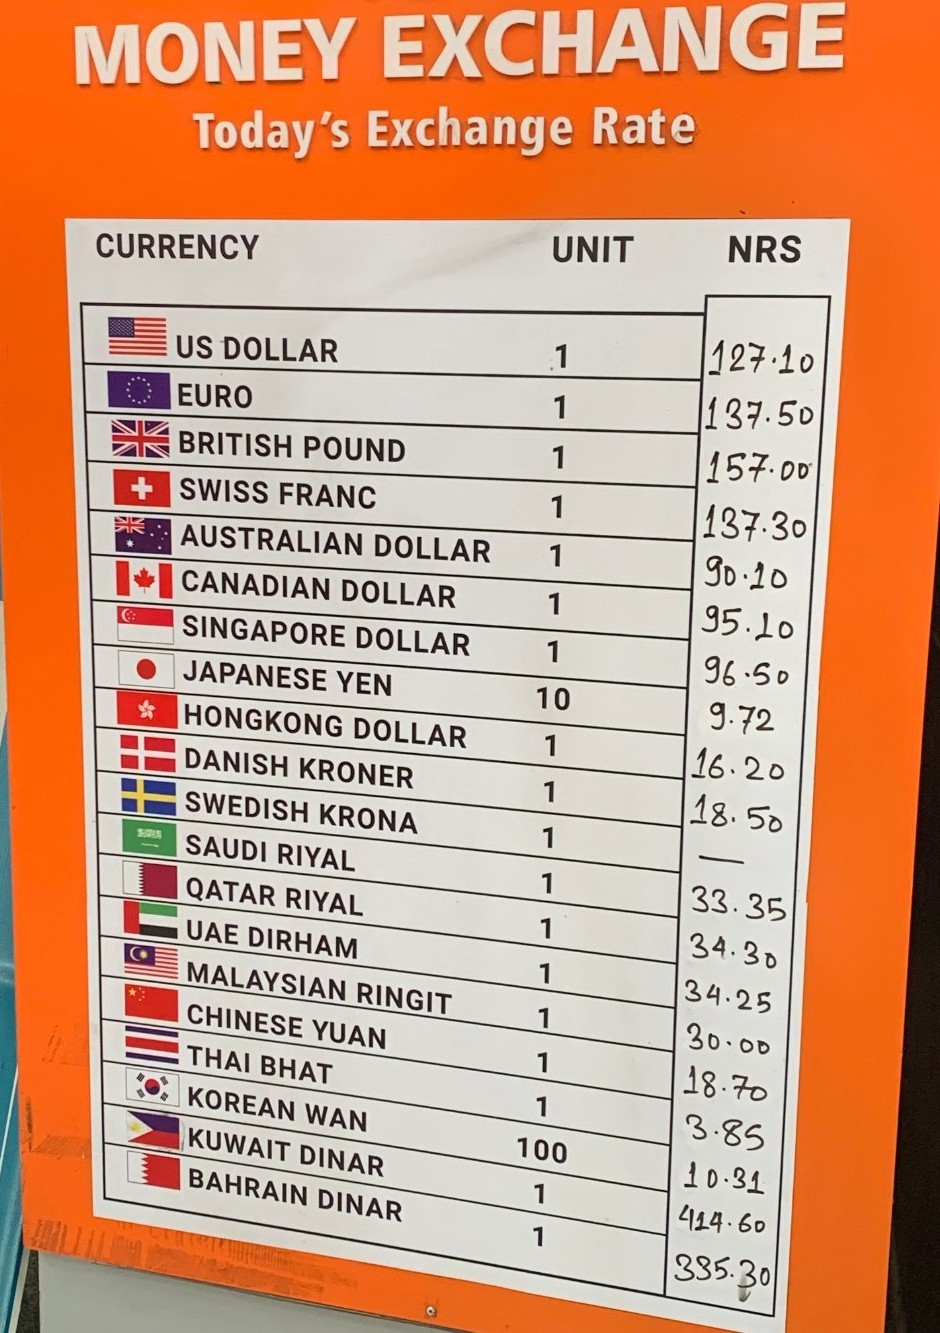
\includegraphics[width=\linewidth]{images/kathmandu_board.jpg}
  \end{minipage}\hfill
  \begin{minipage}[c]{0.56\linewidth}
    \caption{Exchange board at Kathmandu airport, January 2023.}
    \label{fig:m1-board}
    \small\sffamily
    Each row is a direct quote in Nepalese rupees (NRs). A US dollar costs NRs~127.10 and a UAE dirham, the currency Ravi earns, about NRs~34.
    \figsource{Photograph by Chainwit, \href{https://commons.wikimedia.org/wiki/File:Arrival_at_Kathmandu_Tribhuvan_Airport_(01-2023)_-_img_06.jpg}{Wikimedia Commons}, \href{https://creativecommons.org/licenses/by/4.0/}{CC BY 4.0}, cropped.\cite{chainwit2023}}
  \end{minipage}
\end{figure}

\begin{didyouknow}{Every board hides two prices}
A bank buys a currency from you at a lower rate and sells it to you at a higher one. Suppose it buys dollars at ₹93.50 and sells them at ₹96.50. Then ₹10,000 buys US\$103.63, which sells straight back for only ₹9,689. The missing ₹311 is the bank's earning, the \textbf{spread}. Spreads are widest for cash at airport counters.

(The rates are hypothetical.)
\end{didyouknow}

The rupee is watched mostly against the US dollar, the world's working currency, which was on one side of 89 per cent of all currency trades in April 2025.\cite{bis2025} Crude oil, India's biggest import, is priced in dollars, and only about 6 per cent of India's exports are invoiced in rupees,\cite{rbi2026a} even though the Reserve Bank of India (RBI) has allowed trade to be settled in rupees since July 2022.\cite{rbi2022} The dollar even reaches the UAE dirham, which has been fixed, or \textbf{pegged}, at 3.6725 per US dollar since 1997\cite{nagraj2024} \seesec{sec:systems}. So when a dollar costs more rupees, so does every dirham Ravi sends home.
